\documentclass[a4paper,12pt]{extarticle}

\renewcommand{\baselinestretch}{1.1}
\setlength{\parindent}{0cm}

%%% Add packages here
\usepackage{times}
\usepackage[utf8]{inputenc}
\usepackage{graphics}
\usepackage{graphicx}
\usepackage{lscape}
\usepackage{amsfonts}
\usepackage{amsmath}
\usepackage{amsthm}
\usepackage{array}
\usepackage{amssymb}
\usepackage{latexsym}
\usepackage{verbatim}
\usepackage{color}
\usepackage{xcolor}
\usepackage{fancyhdr}
\usepackage{fancybox}
\usepackage{mathtools}
\usepackage{graphics}
\usepackage{nameref}
% folowing  must be in this order
\usepackage{varioref}
\usepackage[colorlinks,citecolor=black,linkcolor=black]{hyperref}
%\usepackage{subfig}
\usepackage{subcaption}
\usepackage{setspace}
\usepackage{lineno}

%\usepackage{w-thm}

\usepackage[comma,sort&compress]{natbib}
\bibliographystyle{apalike}
\usepackage{float}
\usepackage[utf8]{inputenc}
\usepackage[english]{babel}
\usepackage{multicol}

\addtolength{\oddsidemargin}{-.50in}
\addtolength{\evensidemargin}{-.50in}
\addtolength{\textwidth}{1.0in}
\addtolength{\topmargin}{-.40in}
\addtolength{\textheight}{0.80in}

\pagestyle{fancy}
%\chead{\groupname}
\rhead{cyanoFilter: }
\lhead{O. Oluwafemi \textit{et al.}}
\cfoot{\thepage}
\renewcommand{\headrulewidth}{1.9pt}

\begin{titlepage}
	\title{
		\begin{flushleft} 
			\Huge{cyanoFilter: an R package to identify phytoplankton population contained in flow cytometry data using cell pigmentation and/or complexity.} \\
			\vspace{0.4in} \small{Oluwafemi D. Olusoji$^{1,2}$, Jurg W. Spaak$^{2}$, Mark Holmes$^{2}$, Thomas Neyens$^{1}$, Marc Aerts$^{1}$, Frederik De Laender$^{2}$} \\\vspace{0.2in}			
			$^{\text{\sf 1}}$Centre for Statistics, Data Sceince Institute, Hasselt University, Hasselt, 3500, Belgium\\
			$^{\text{\sf 2}}$Research Unit in Environmental and Evolutionary Biology (URBE), Institute of Life-Earth-Environment (ILEE), Namur Institute for Complex Systems (NAXYS), Universit\'{e} de Namur, Namur, 5020, Belgium.\\\vspace{0.2in}
			\textbf{Contact:}\\ \href{oluwafemi.olusoji@uhasselt.be}{oluwafemi.olusoji@uhasselt.be}\\
			\textbf{Supplementary information:} Supplementary data are available at \textit{}
		\end{flushleft}
	}

	\date{}
\end{titlepage}


\begin{document}
	
	\maketitle
	\newpage
	\linenumbers
	\begin{abstract}
		\textbf{Summary:} 
		\begin{enumerate}
			
			\item Flow cytometry is often employed in Ecology to measure traits of primary producers such as phytoplankton. This technique offers the advantages of speed since millions of particles can be measured in relatively small amount of time. However, scientists often face the problem of differentiating the different outcomes that can result from such measurements to the particles that are of interest.
			
			\item Gating is the process of identifying particles measured in flow cytometry (FCM). This process could either be manual, where particles are identified using known characteristics of these particles, or automated, where automated clustering techniques are employed to identify and group these particles. Available automated gating frameworks implemented in statistical packages for flow cytometry are primarily developed for identifying outcomes in human FCM experiments with only two of such existing for cyanobacteria.
			
			\item cyanoFilter is an R package built to identify phytoplankton populations from flow cytometry data, based on a reproducible semi-automated gating framework. The algorithm uses pigment information about the phytoplankton cells to gate out the respective population.
			
			\item Source code is freely available through the Comprehensive R Archive Network (CRAN) \href{https://cran.r-project.org/web/packages/cyanoFilter/index.html}{https://cran.r-project.org/web/packages/cyanoFilter/index.html}. Some experiment data is made available in package. 
			
		\end{enumerate}

		\noindent \textit{Keywords: }
	\end{abstract}


\title{}
%\author[Sample \textit{et~al}.]{Oluwafemi D. Olusoji\,$^{\text{1,2,}*}$, Jurg W. Spaak\,$^{\text{2}}$, Frederik De Laender\,$^{\text{2}}$, Thomas Neyens\,$^{\text{1}}$ and Marc Aerts\,$^{\text{1}}$}
%\address{}

\maketitle

\doublespacing

\section*{Introduction}
Phytoplankton are primary producers responsible for about 50\% of global production. \emph{Synechococcus} cyanobacteria, a common component of the phytoplankton community, are one of the known oldest life forms known to perform photosynthesis. They are ubiquitous worldwide \citep{Dvorak:2004}, and are at the base of many aquatic food webs \citep{Kirk:1994}. Although phytoplankton compete for a small number of resources (e.g. light, nitrogen, phosphorus), a dozen number of different phytoplankton species are often found together. One of the possible explanations for this is the partitioning of the light spectrum \citep{Stopm:2004}. For example, \cite{Stopm:2004} identified two species of picocyanobacteria from the Baltic sea; \emph{BS4} and \emph{BS5} that uses phycocyanin to absorb red light and phycoerythrin to absorb green light respectively.

Recently, studies seeking to better understand the ecology of phytoplankton in general employed flow cytometry (FCM) to measure phytoplankton abundance \citep{Pomati:2013, Stopm:2007, Fontana:2018}. Although there are earlier applications of FCM to measure cyanobacteria cells in ecology \citep{Trask:1982a, Berglund:1988}, the emergence of microbial ecology alongside the possibility of obtaining individual level data that can enhance the understanding of community assembly and biodiversity drives its current use \citep{Fontana:2014a}. 

FCM is a technique that involves the suspension of cells or particles within a fluid stream which is made to pass through one or more laser beams \citep{ONeill:2013}. A crucial step in FCM application is to separate signal from noise, e.g. phytoplankton cells from other particles, including debris. Gating or clustering is the classical approach taken in FCM to meet this challenge: measured particles are classified based on their properties, most notably how they reflect and/or absorb light. This process can be done manually, termed manual gating or with the use of automated algorithms in computer software packages, termed automated gating \citep{ONeill:2013}. We must also note that some flow cytometers are already equipped with cell sorters which can automatically differentiate between phytoplankton cells based on properties such as; cell morphology, cellular physiology and taxonomic positions \citep{Ibrahim:2007}. However, such machines are not without shortcomings \citep{Sinigalliano:2009}. 

Frequently, identification of phytoplankton cells, i.e gating, in FCM experiments is done manually with software like; FCS Express \href{https://
	www.denovosoftware.com/}{(https://
	www.denovosoftware.com/)}, FloMax \href{https://www.sysmex-partec.com/}{(https://www.sysmex-partec.com/)}, flowJo \href{https://www.flowjo.com/}{(https://www.flowjo.com/)}, Incyte \href{https://www.luminexcorp.com/guava-easycyte-flow-cytometers/\#software}{(https://www.luminexcorp.com/guava-easycyte-flow-cytometers/\#software)}, model based tools such as; \texttt{flowClust} \citep{Lo:2009} and \texttt{flowEMMi} \citep{Ludwig:2019} or machine learning \citep{Fontana:2018}. Manual gating is often not reproducible, while model based tools require tuning of global parameters that are not related to the biological properties of the measured cells, plus it is often difficult to include experts knowledge with this approach\citep{Malek:2015a}. To remedy these, we introduce the R package \emph{cyanoFilter} for gating phytoplankton FCM data. The package offers a semi-automated gating approach of phytoplankton FCM experiments by using pigment information to identify each phytoplankton population contained in FCM data. Aside from identifying phytoplankton populations, \emph{cyanoFilter} can also help identify previously unknown light channels that can help differentiate phytoplankton cells.


%, which paves the way for joint analysis of these outcomes. %Furthermore, the package contains tools for FCM data pre-processing and visualisation.
%\enlargethispage{3pt}
%\vspace*{-8pt}
%\section{Approach}
 %The first step addresses the question of the appropriate dilution level, the second step addresses the need for transformation or not, next the transformation is evaluated, and the last two steps address the identification of the different FCM outcomes and the cyanobacteria populations. If the transformation is not needed, the process moves to the last two steps. The process of identifying these outcomes requires the knowledge of both the flow cytometer light channels and properties of the measured cells. 
\section*{Materials and Methods}

\begin{figure}[t] 
	
	\centering
	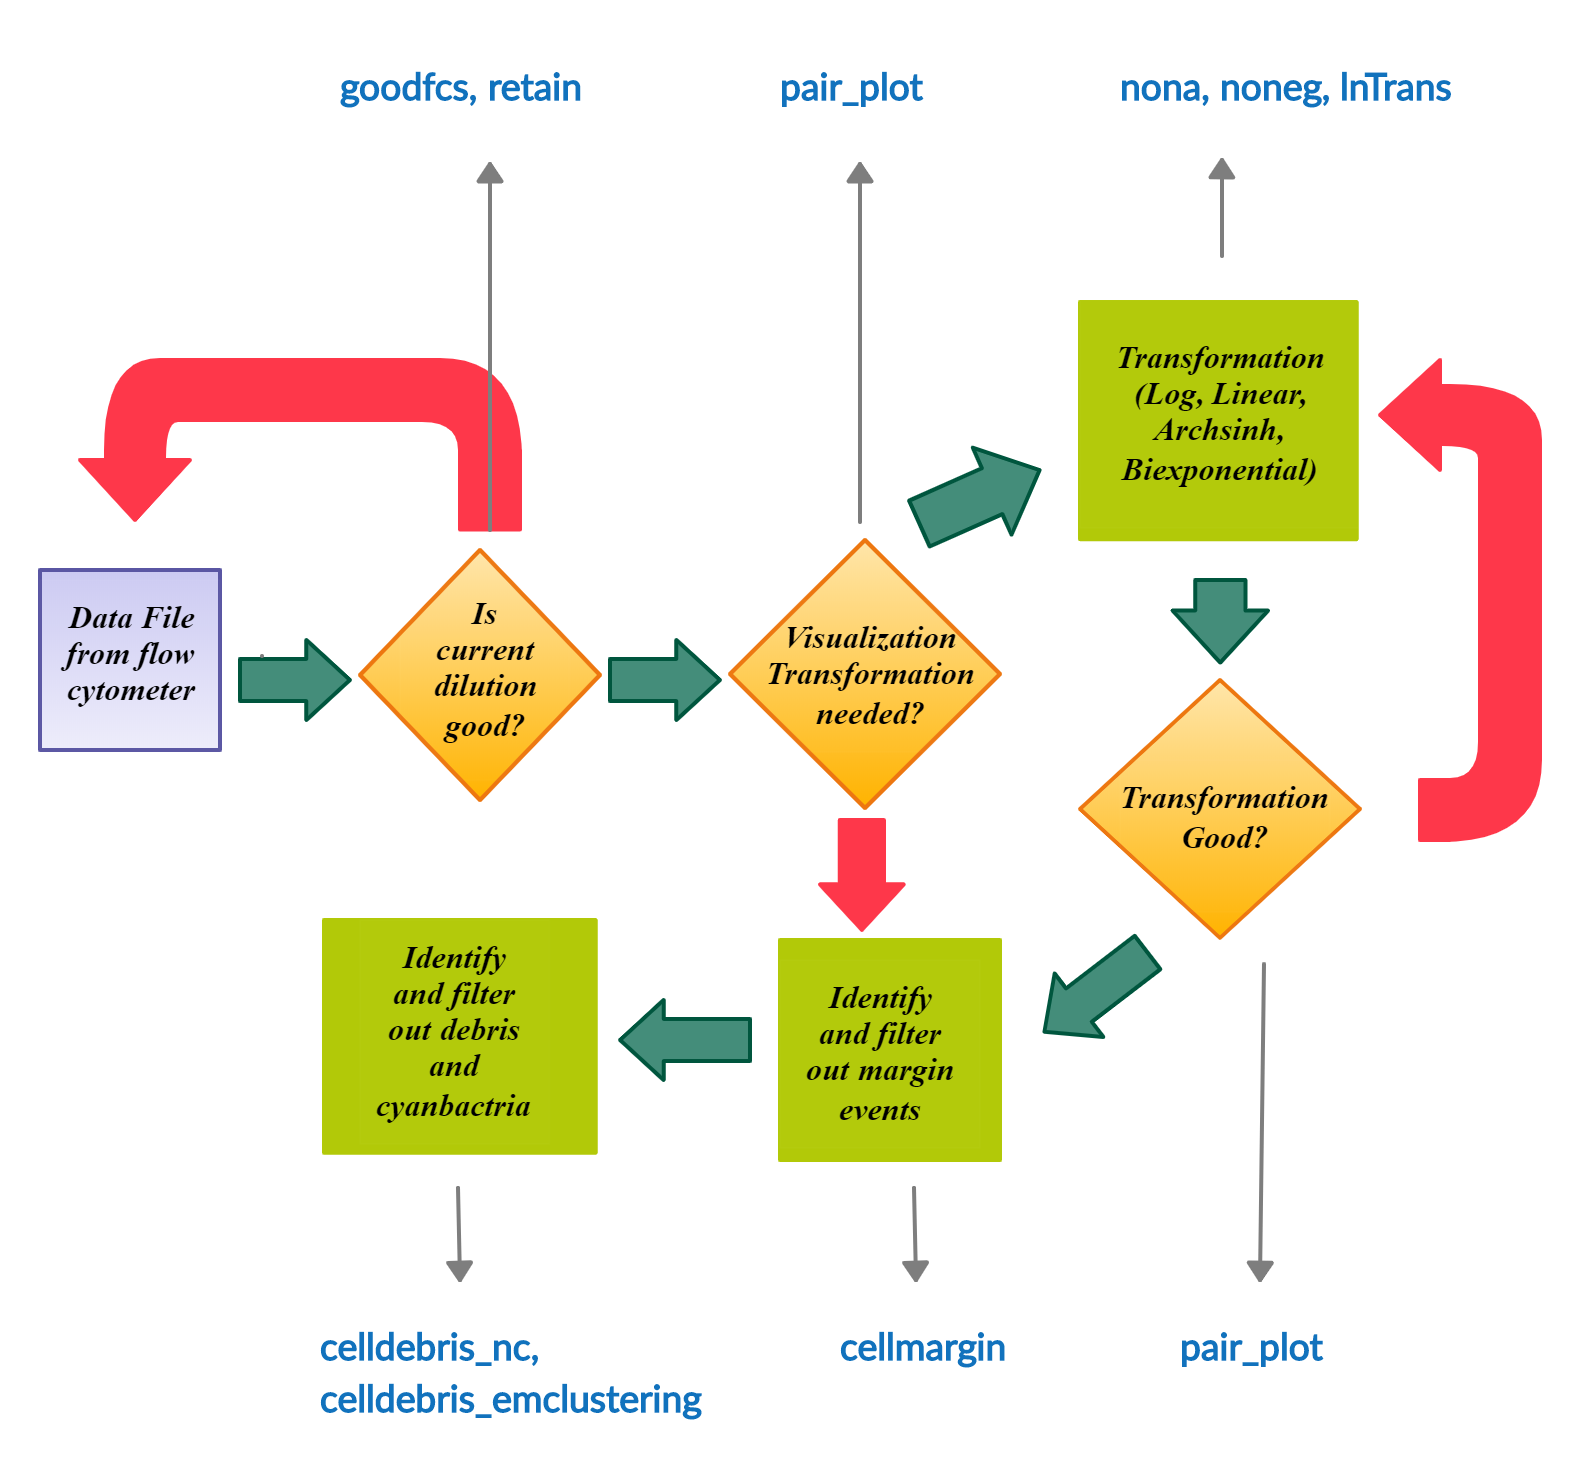
\includegraphics[scale = 0.2]{Figures/software_framework.png}
	\caption{cyanoFilter Framework. A green arrow implies a positive answer to the question posed in the rhombus while a red arrow implies a negative answer. The black arrows are pointing to functions within the package that perform the required tasks at each level.}
	\label{fig:framework}
\end{figure}

The purpose of \texttt{cyanoFilter} is to provide a simple to use set of tools that uses pigment information to identify phytoplankton population contained in FCM experiments. This makes it an alternative to manual gating, machine learning and electron microscopy which is often employed to identify phytoplankton population in FCM experiments \citep{Stopm:2007, Fontana:2017, Poniedzialek:2017}.

FCM experiments result in four outcomes, namely: debris, margin events, multiplets and singlets. Debris are residues and non-living cells that are not of interest, margin events are particles larger than the maximum width measurable by the flow cytometer while multiplets are two or more particles stuck together. Singlets are the good cells that can be further explored and divided into different phytoplankton populations. The process of properly identifying these outcomes requires the knowledge of both the flow cytometer light channels and properties of the measured cells.

Figure \ref{fig:framework} presents the framework guiding \texttt{cyanoFilter}. This framework is a full pipeline of phytoplankton FCM analysis assuming the correct dilution is not known beforehand. 

The central algorithm in \texttt{cyanoFilter} uses the minimum intersection point between peaks identified in one dimensional kernel density evaluated along supplied pigment and/or cell complexity channels to partition particles into different groups. This approach to clustering FCM data is documented in \cite{Malek:2015a}. After the initial partitioning per channel, we assign unique labels to each group. Then all possible combinations of the labels are formulated and re-labelled as potential clusters. The algorithm then tries to retain a proportion of the total number of particles clustered. We included this option because the process of forming all possible combinations after the partitioning step often lead to clusters with a small number of particles that the algorithm could not properly classify. The idea of using pigmentation of phytoplankton to differentiate them is not new. This idea is central to microscopy. To summarise, the clustering is carried out in the following steps;

\begin{enumerate}
	\item Search for peaks and the minimum intersection points between these peaks across the supplied pigment and cell complexity channels.
	\item Divide particles into groups based on the minimum intersection points identified in 1 and label each group.
	\item Formulate all possible combinations of labels in 2.
	\item Assign a new label to the combinations in 3.
	\item Retain clusters that make up a desired proportion of the total number of particles clustered.
\end{enumerate}

Flow cytometers come with a channel dedicated to measuring the width of every particle measured, making it possible differentiate margin events from the rest. We use step 1 and 2 of the algorithm described above to separate margin from non-margin events since it involves only one channel. 

Also, flow cytometers come equipped with tools to ensure the avoidance of multiplets during the acquiring phase of the measuring process. Hence, identifying them is not addressed in \texttt{cyanoFilter}.


\subsection*{Implementation}

\texttt{cyanoFilter} is written entirely in \textbf{R} \citep{r:2016}, and it offers functions to process standard FCS files. There are functions to visualise and cluster phytoplankton population contained in a FCS file. See table \ref{table:func} for a list of the main functions in the package. All clustering functions produce two-dimensional (2D) graphs by default for users to evaluate the performance of the algorithm.

\begin{table}[t] 
	\centering
	\begin{tabular}{ll}
	\hline
	Function & Description \\
	\hline
	\texttt{goodfcs} & identifies FCM experiments measured at the appropriate dilution using \\
	& supplied desired minimum and maximum $cell/\mu l$.\\ 
	& Useful for dilution series measurements.\\
	\texttt{ggpairsDens} & scatter plot matrix of measured cells along the supplied channels\\
	\texttt{ggplotDens} & scatter plot of measured cells along two channels\\
	\texttt{cellmargin} & removes margin events from supplied FCS\\ & file based on Side Scatter Width (SSC.W) by default\\
	\texttt{pigment\_gate} & calls the gating algorithm on the pigment channels\\
	\texttt{complexity\_gate} & calls the gating algorithm on the cell complexity channels\\
	\texttt{phyto\_filter} & top level function to call pgiment\_gate and complexity\_gate\\
	\texttt{cluster\_summary} & provides a basic statistical summaries of a cluster\\
	\texttt{cluster\_extract} & extract specific cluster of interest based on supplied label\\
	\hline
	\end{tabular}
\caption{Main functions in \texttt{cyanoFilter}}
\label{table:func}
\end{table}

\subsubsection*{Installation}
The \texttt{cyanoFilter} \textbf{R} package is available on the Comprehensive \textbf{R} Archive Network (CRAN) at \url{https://cran.r-project.org/web/packages/cyanoFilter/index.html}. The package and its bioconductor (\url{https://bioconductor.org/}) dependencies; \texttt{Biobase}  \citep{biobase:2015}, \texttt{flowCore} \citep{flowCore:2019}, and \texttt{flowDensity} \citep{Malek:2015a} can be installed and loaded using the following commands:\\
\texttt{install.packages("BiocManager")\\
	library(BiocManager)\\
	install(c("flowCore", "flowDensity", "Biobase"), update = FALSE)\\
	install.packages("cyanoFilter", dependencies = TRUE)\\
	library(cyanoFilter)
}



%For FCM experiments conducted using dilution series, identifying files measured at the appropriate dilution level is often of interest. The \texttt{goodfcs()} function uses the desired minimum, maximum $cell/\mu l$ to identify these files. The function adds an extra column (\texttt{Status}) with the entry \texttt{good} or \texttt{bad} to the metafile. Rows containing cell/$\mu l$ values outside the desired minimum and maximum are labelled \texttt{bad}. The \texttt{retain} function can further help identify the file with the highest (or smallest) cell/$\mu l$ among the appropriately measured files.

%\vspace*{-0.1in}

%The \texttt{pair\_plot} function produces a panel plot of all measured channels. Each plot is also smoothed to show the cell density. The \texttt{nona} and \texttt{noneg} function helps remove \texttt{NA}'s and negative values contained in the measured channels. We provide a function for the natural logarithm transformation (\texttt{lnTrans}). Other possible  transformation functions can be found in the  \texttt{flowCore} package.

%\vspace*{-0.1in}

%To remove margin events, the \texttt{cellmargin} function takes the column in the expression matrix corresponding to measurements about the width of each cell. It returns a figure (supplementary material) and a list containing a R FCM file (flowframe) with non-margin events, a flowframe containing all particles with an indicator for margin and non-margin events, the number of margin and non-margin events.

%\vspace*{-0.1in}

%The \texttt{celldebris\_nc} and \texttt{celldebris\_emclustering} functions require two and at least two channels respectively, each characterising cyanobacteria properties, to separate debris from cyanobacteria populations. The functions identify cyanobacteria using \emph{flowDensity} \citep{Malek:2015a} and \emph{finite-mixture} approach \citep{Lo:2009} respectively. Both functions return a figure (right figure in Figure~1\vphantom{\ref{fig:1}} and supplementary material) showing the clusters. In addition, \texttt{celldebris\_nc} returns a list containing the following: i) a flowframe with all debris removed, ii) a flowframe with all measured particles with an indicator for debris and cyanobacteria cells, iii) the number of cyanobacteria cells counted, and iv) the number of debris particles counted, and \texttt{celldebris\_emclustering} returns the following: i) final weight for each cluster, ii) a matrix of means for each channel per cluster, iii) a list containing variance-covariance matrices for each cluster, iv) a flowframe containing all the measured particles and the associated probabilities.

 
 \section*{An Example}
 
 To illustrate the functionality of the package, we ran a flow cytometry experiment on 5 species of cyanobacteria. First, we apply cyanoFilter on the monoculture experiments involving each of this species. Then, we also apply cyanoFilter on bi-culture experiments containing all unique combinations of the species. Table \ref{table:strains} displays information about the strains and their pigmentation. We supplied RED.B.HLin, YEL.B.HLin, RED.R.HLin which measures the presence of chlorophyll \textit{a}, phycoerythrin and phycocyanin respectively as pigment channels, while we supplied FSC.HLin and SSC.HLin which measures size and cell complexity respectively as complexity channels.
 
 \begin{table}[t] 
 		\centering
 			\begin{tabular}{ccc}
 				\hline
 				Species 1 & Species 2 & Pigment (Species 1, Species 2)\\
 				\hline
 				2524 & 2434 & 2,1\\
 				2375 & 2434 & 2,1\\
 				2555 & 2434 & 1,1\\
 				2385 & 2434 & 3a,1\\
 				2380 & 2434 & 3a,1\\
 				2375 & 2524 & 2,2\\
 				2555 & 2524 & 1,2\\
 				2385 & 2524 & 3a,2\\
 				2380 & 2524 & 3a,2\\
 				2555 & 2375 & 1,2\\
 				\hline
 		\end{tabular}
 	\caption{Names and pigmentation of the species used in the experiments.}
 	\label{table:strains}
 \end{table}
 
 
 \subsubsection*{Metafile pre-processing}
 R code about pre-processing here
 \subsubsection*{Transformation and visualisation}
 R code about transformation and visualisation here
 \subsubsection*{Gating margin events}
 R code about gating margin events here
 \subsubsection*{Gating debris and phytoplankton}
 R code about gating debris and phytoplankton here
 
 \section*{Limitation}
 
 \begin{figure}[t] 
 	\centering
 	\begin{subfigure}{0.48\linewidth} \centering
 		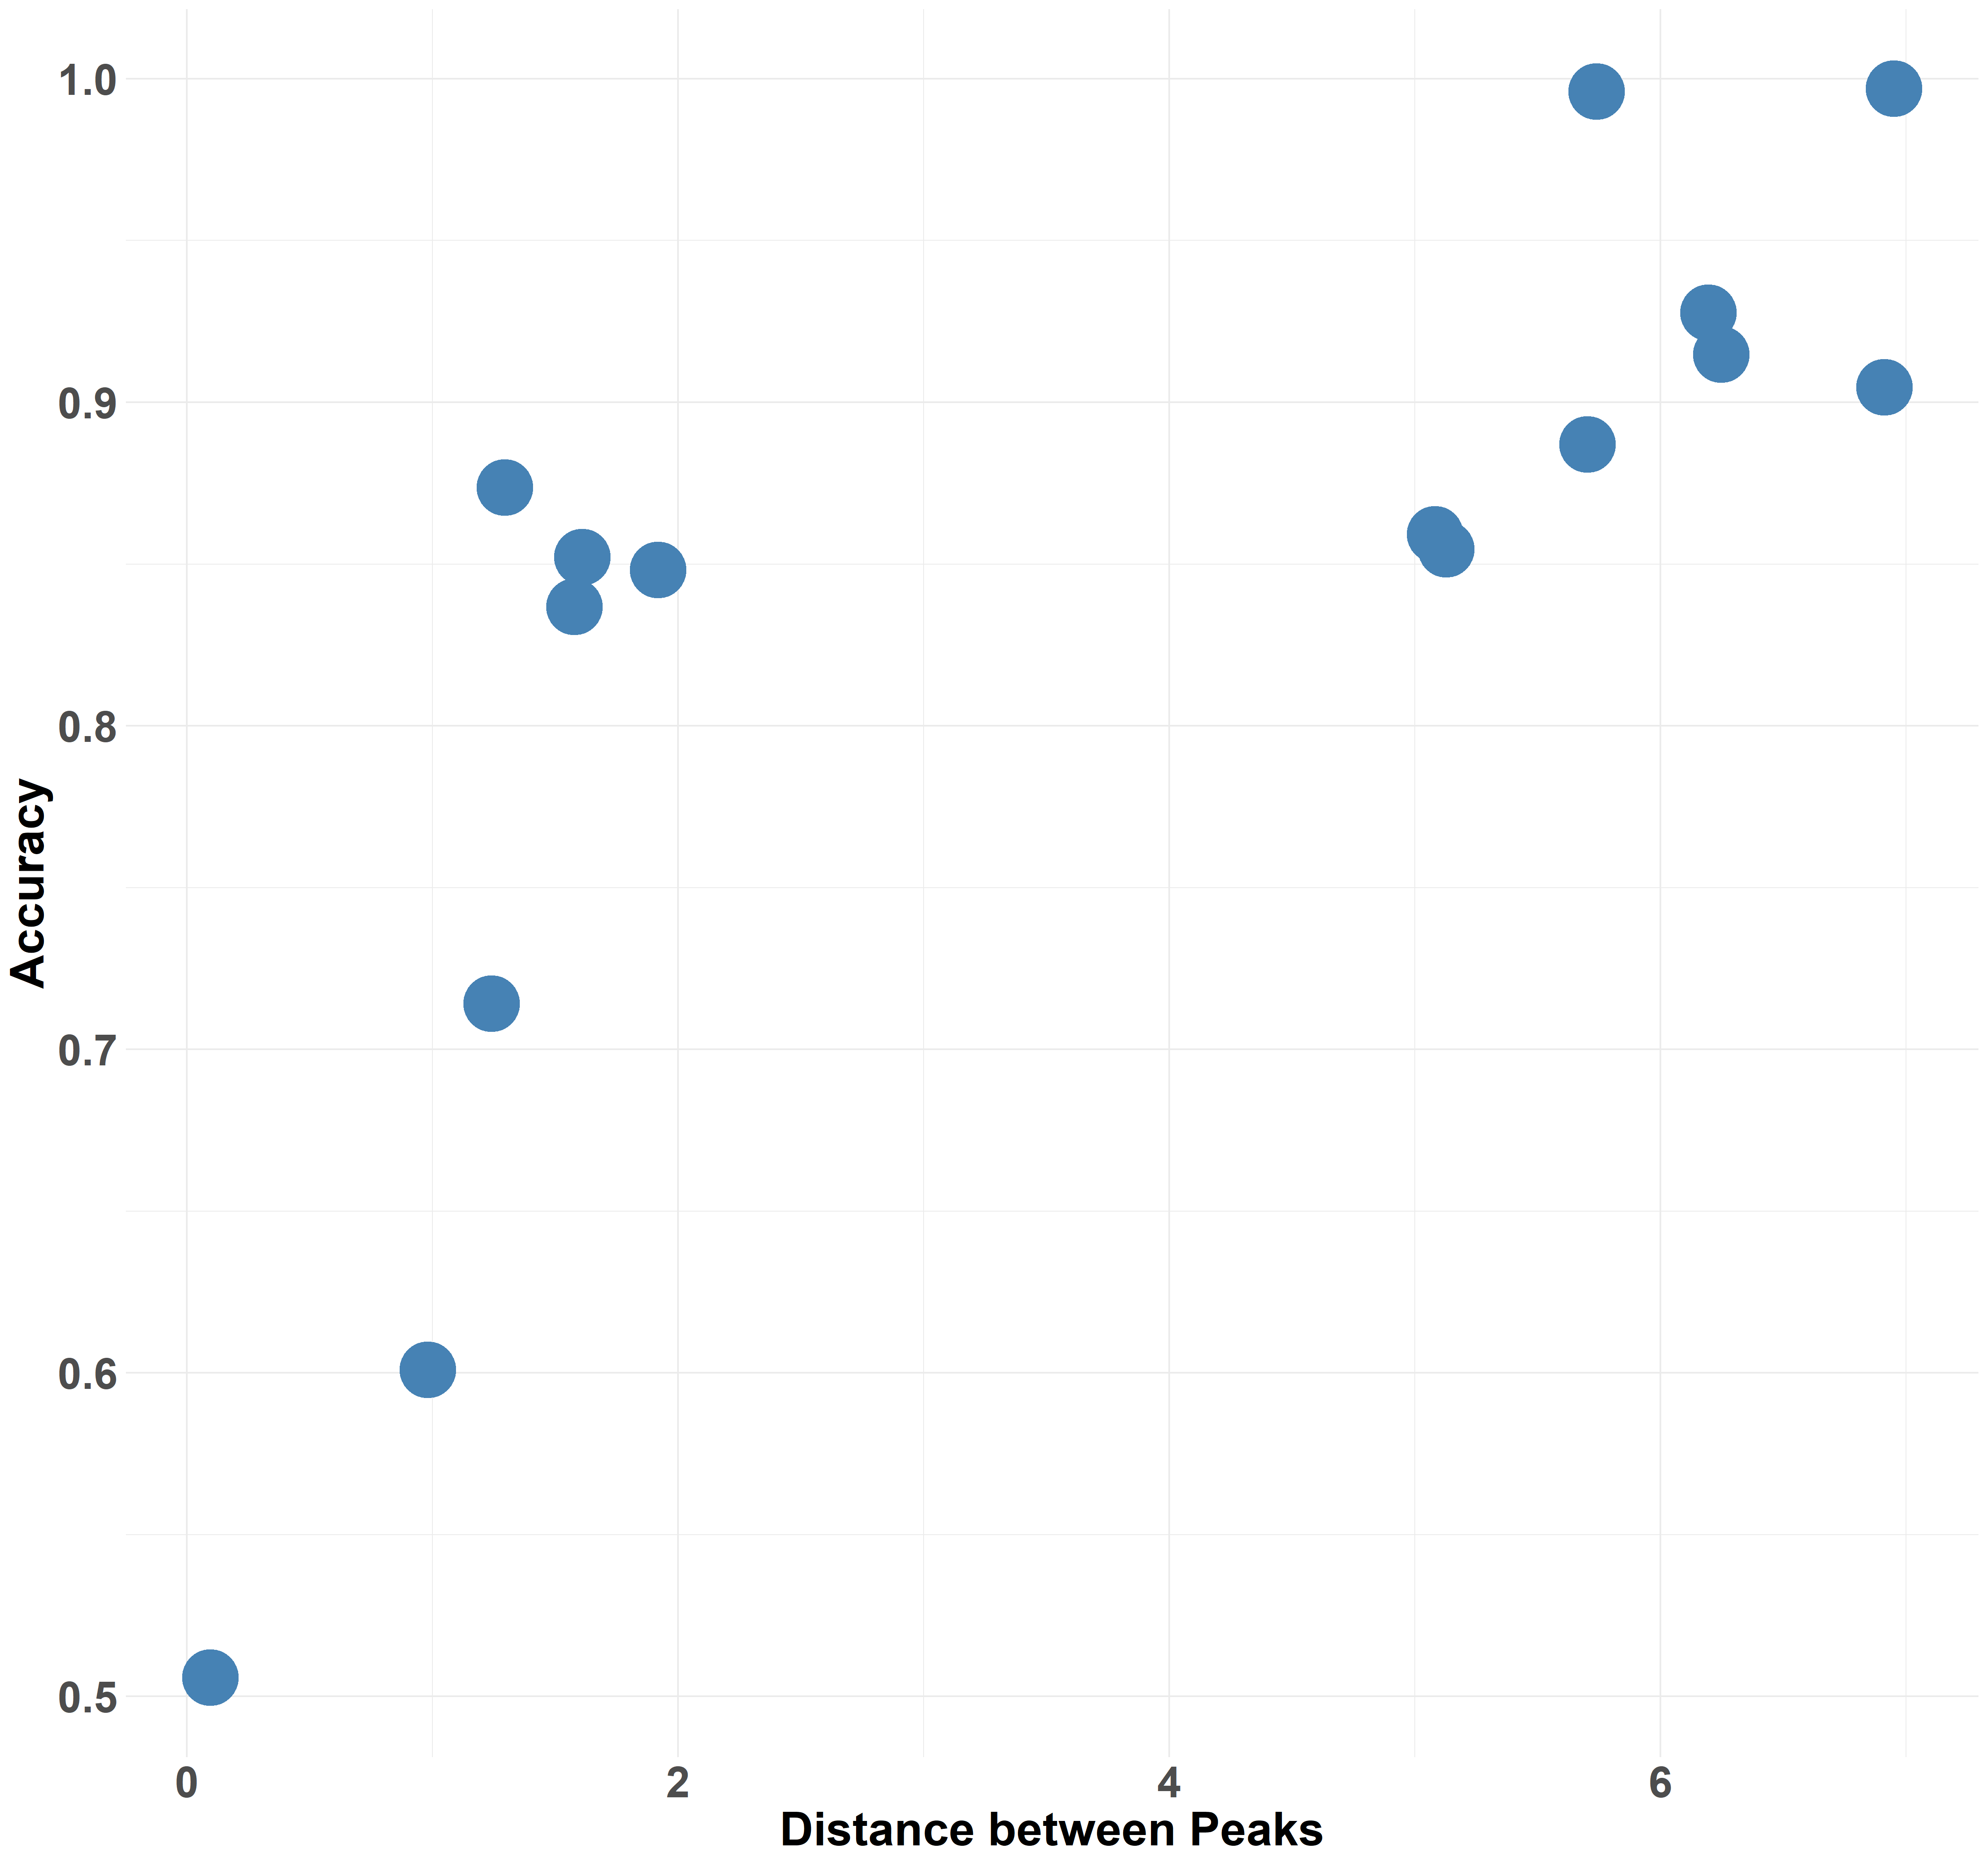
\includegraphics[scale = 0.2]{Figures/AccuracyPlot_Distance.png}
 		\caption{}
 	\end{subfigure}
 	\begin{subfigure}{0.48\linewidth} \centering
 		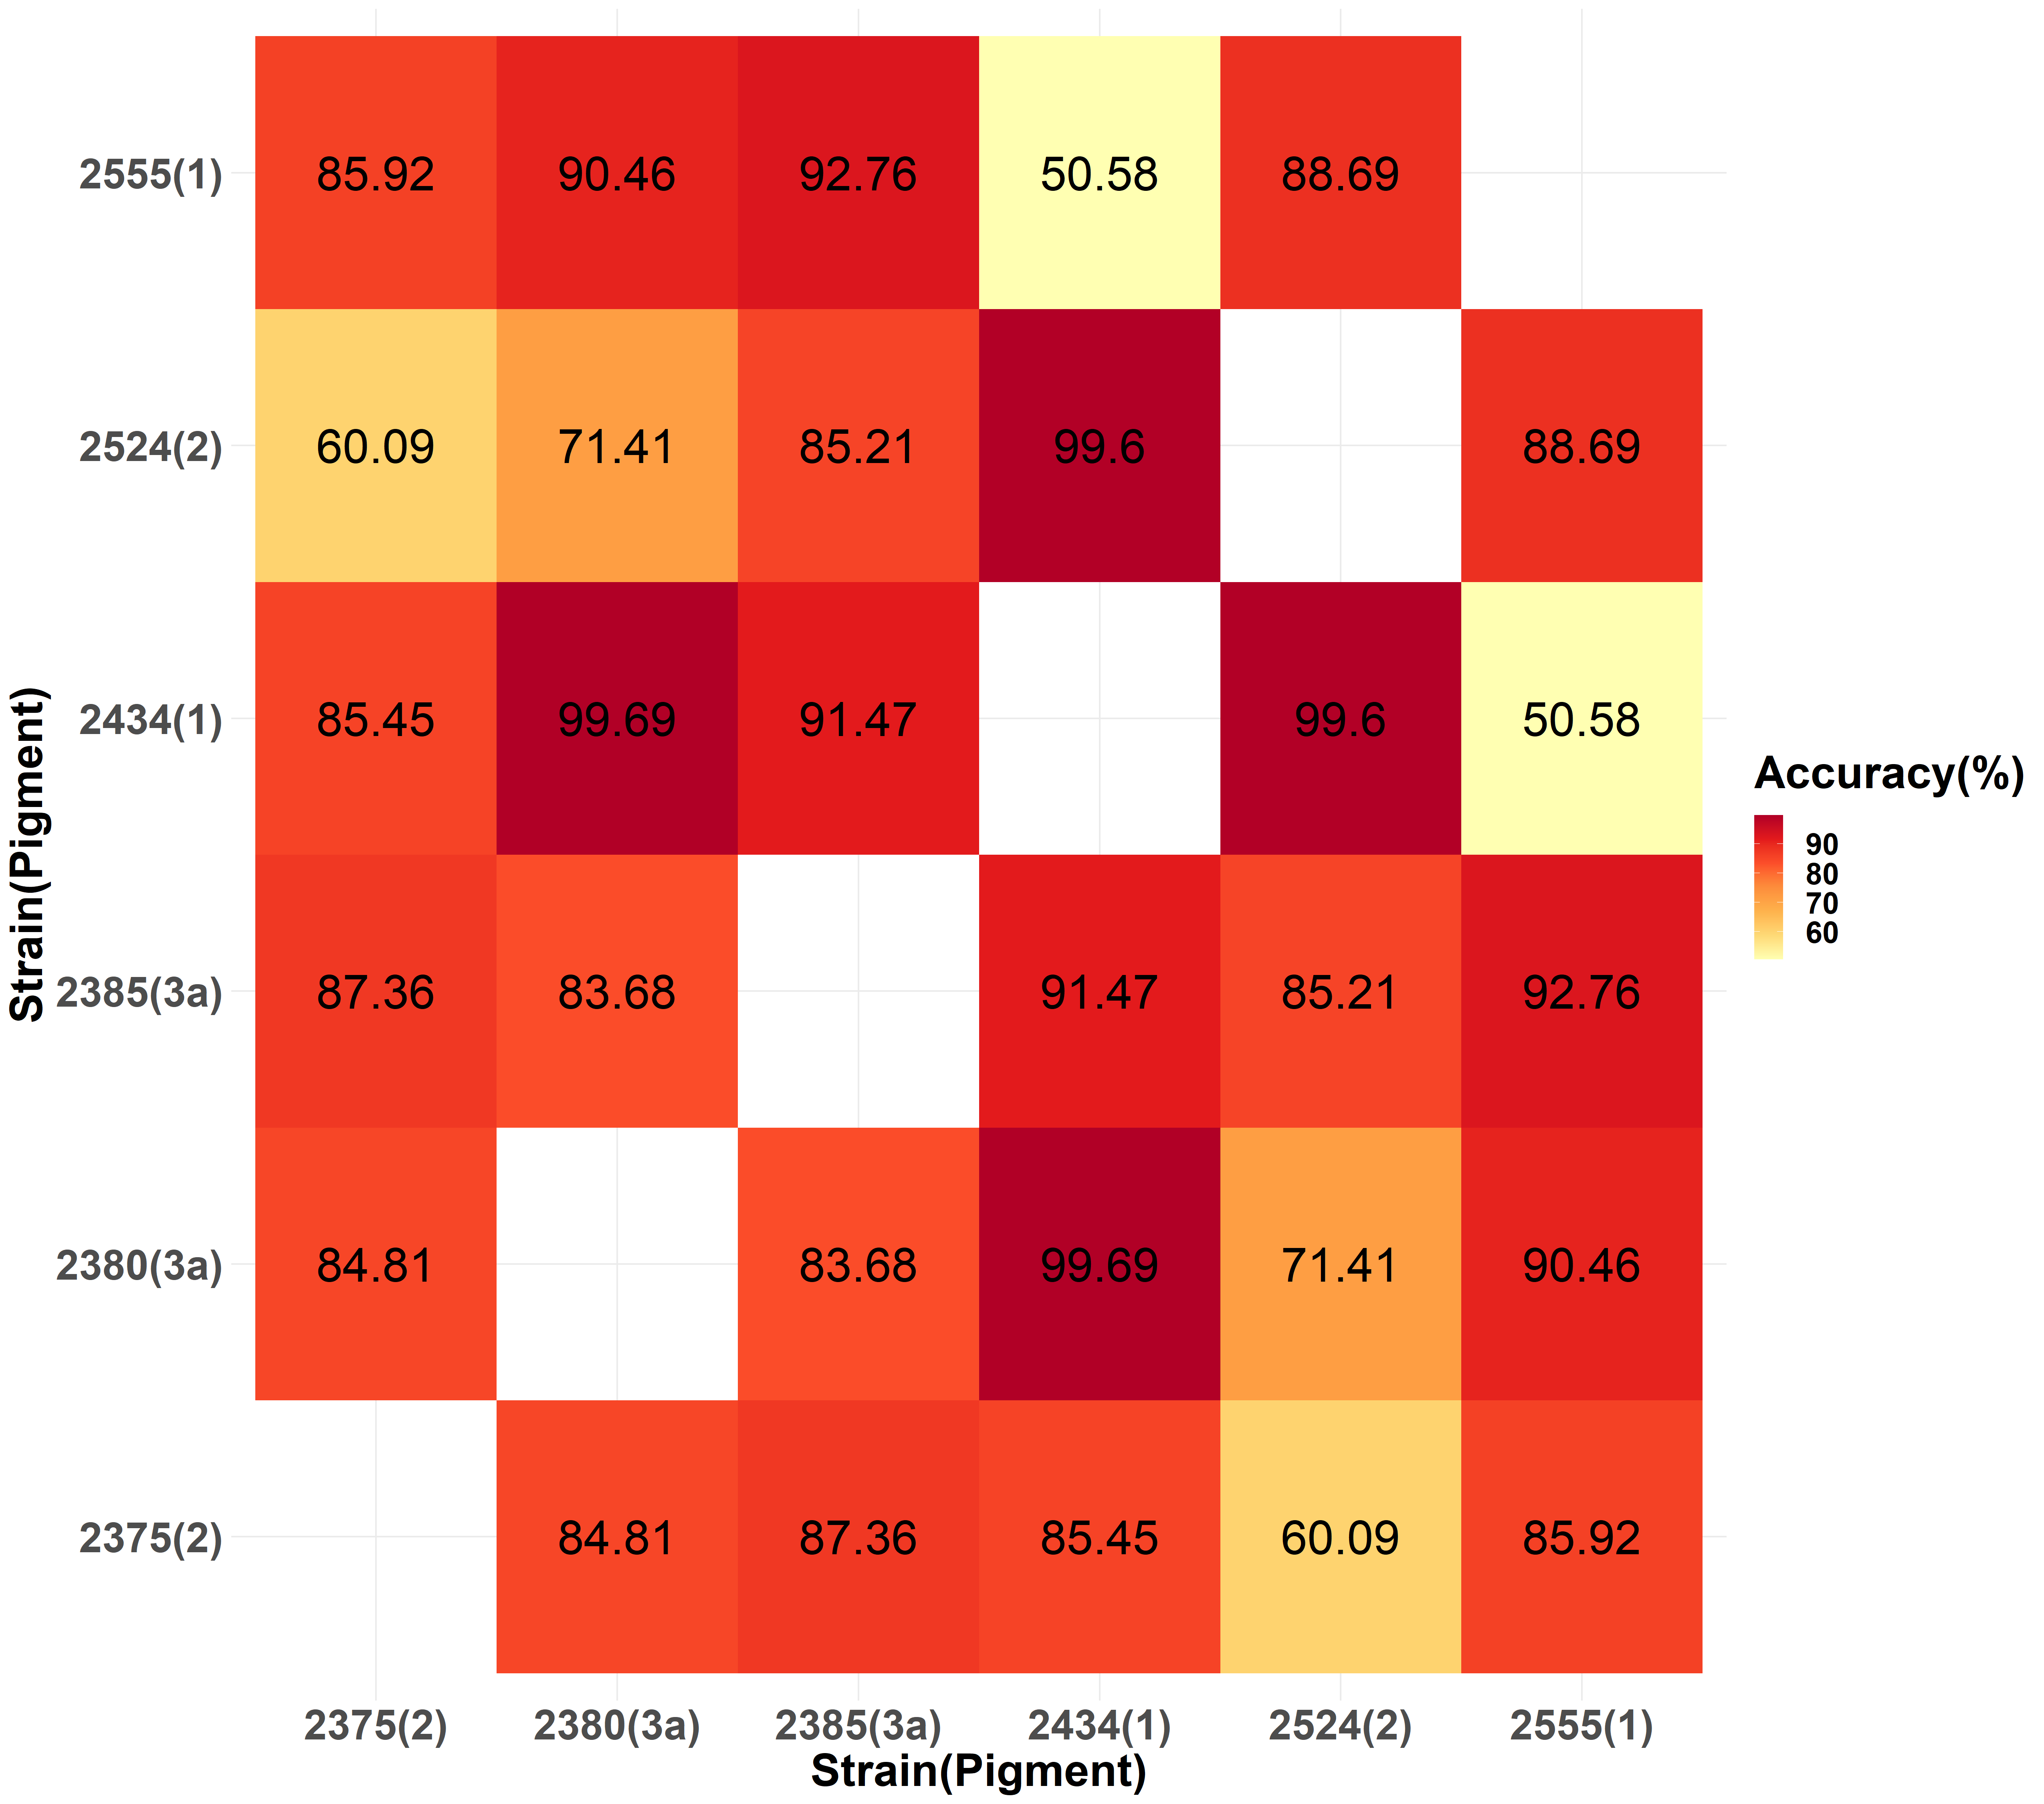
\includegraphics[scale = 0.2]{Figures/AccuracyPlot.png}
 		\caption{}
 	\end{subfigure}
 	\caption{(a) Accuracy as against the Euclidean distances between the peaks observed along the pigment and cell complexity channels. (b) Accuracy by species and their pigmentation.}
 	\label{fig:results}
 \end{figure}
 
 The example illustrated above provides us with data to evaluate the performance of the central algorithm in \texttt{cyanoFilter}. To do this, we employed a resampling scheme where we examined the label assigned to every two randomly sampled cells after applying \texttt{cyanoFilter} on the monoculture and bi-culture experiment described in table \ref{table:strains}. If the algorithm assigns the same label to the sampled cells in monoculture, i.e. similar cells, we expect the same outcome if we examine the labels of these cells in the bi-culture experiment. Therefore, assigning similar or different labels to the same sampled cells in the monoculture and bi-culture experiment meant agreement, while dissimilar labels meant otherwise. We repeat this ten thousand times to enable us compute a measure of accuracy. We define accuracy as the number of times the algorithm agrees between the labels in the monoculture and bi-culture experiments per ten thousand resample. Figure \ref{fig:results} presents the result of this exercise. We observe that the accuracy increases with increasing distance between detected peaks. Thus, for phytoplankton species with pigments absorbing light at differing peaks, the algorithm will properly classify such species. However, it will suffer if the species under consideration have pigmentation that absorb light at similar peaks. 
 
 
\section*{Summary}
 \emph{cyanoFilter} offers a suite of functions that helps with pre-processing of FCM files and identification of all outcomes therein. It can gate cyanobacteria FCM experiments with the advantage of easy integration of knowledge about the measured cells (users can supply channels containing such information as options) and reproducibility (steps documented as R codes).
 
\section*{Authors' Contributions}
Marc Aerts, Frederik De Laender and Thomas Neyens applied for the funding for the study that led to the development of the framework and package. Oluwafemi D. Olusoji wrote the manuscript. Marc Aerts, Frederik De Laender, Thomas Neyens and Jurg W. Spaak edited the manuscript.  Oluwafemi D. Olusoji and Jurg W. Spaak developed the algorithm and wrote the corresponding \textbf{R} codes. Mark Holmes performed the experiment that provide data for the examples and evaluation of the algorithm. 
 
\section*{Acknowledgements}
Many thanks to several productive discussions with Jurgen Claesen on several aspects of the package.

\section*{Funding}
This work was supported by funds from the bilateral co-operation (BOF) between Hasselt University and Universit\'{e} de Namur.\vspace*{-12pt}

%\section*{References}

\bibliography{references}
%\begin{thebibliography}{}
	
%\bibitem[Dvorak, 2004]{Dvorak:2004}
%	Dvorak, P. \textit{et~al} (2014) Synechococcus: 3 billion years of global dominance. Mol. Ecol. {\bf 23}, 5538–5551.

%\bibitem[Fontana, 2018]{Fontana:2018}
%Fontana, S. \textit{et~al} (2018) Individual-level trait diversity predicts phytoplankton community properties better than species richness or evenness. ISME Journal {\bf 12}, 2, 356-366.

%\bibitem[Lo, 2009]{Lo:2009}
%Lo, K., Hahne, F., Brinkman, R. et al. (2009) flowClust: a Bioconductor package for automated gating of flow cytometry data. BMC Bioinformatics, {\bf10}, 145.

%\bibitem[Kirk, 1994]{Kirk:1994}
%Kirk, J. (1994) The photosynthetic apparatus of aquatic plants. \textit{Light and Photosynthesis in Aquatic Ecosystems}. 2nd edn., Cambridge University Press, Cambridge.

%\bibitem[Malek, 2015a]{Malek:2015a}
%Malek, M., Taghiyar, M. J. \textit{et~al} (2015) FlowDensity: Reproducing manual gating of flow cytometry data by automated density-based cell population identification. Bioinformatics, {\bf 31}, 606--607.

%\bibitem[ONeill, 2013]{ONeill:2013}
%O'Neill, K., \textit{et~al} (2013) Flow Cytometry Bioinformatics, {\it PLoS Computational Biology}, {\bf 9}, e1003365.

%\bibitem[Pomati, 2013]{Pomati:2013}
%Pomati, F., \textit{et~al} (2013) Individual Cell Based Traits Obtained by Scanning Flow-Cytometry Show Selection by Biotic and Abiotic Environmental Factors during a Phytoplankton Spring Bloom, {\it PLoS ONE}, {\bf 8}, e71677. 



%\bibitem[Ribalet, 2011]{Ribalet:2011} 
%Ribalet, F., Schruth, D. M., Armbrust, V. E.  (2011) flowPhyto: enabling automated analysis of microscopic algae from continuous flow cytometric data, Bioinformatics, {\bf 27}, 5, 732–-733.

%\end{thebibliography}
\end{document}
